\section{Introduction}

Gravitational lensing and dynamical modelling provide independent constraints on the mass distribution of galaxies. Combining them allows for valuable cross-checking opportunities to disentangle the stellar and dark matter (DM) content of galaxies.

Cosmological simulations suggest that cold DM forms cuspy halos following a Navarro-Frenk-White (NFW) profile \citep{NFW96}. However, the existence of central DM density cusps in massive galaxies depends strongly on the stellar mass-to-light ratio (e.g., \citealt{2011MNRAS.416..322D}) and DM dominated dwarf galaxies even favour DM halos with cores (e.g., \citealt{1994Natur.370..629M,2001ApJ...552L..23D}). This discrepancy, known as the core-cusp problem, might be resolved by galaxy formation processes such as mergers and outflows (e.g., \citealt{2001ApJ...560..636E,2012MNRAS.421.3464P}).

Determining the overall mass distribution in massive galaxies and separating the DM from the stellar mass components is therefore a crucial step in better understanding the structure and formation of galaxies and nature of DM.

Massive galaxies can act as gravitational lenses, deflect the light of background sources and give rise to multiple images. This strong gravitational lensing tightly constrains the projected total mass of the lens galaxy inside $\sim 1''$ (e.g., \citealt{2010ARA&A..48...87T}). 

The mass profile at larger galactocentric radii can be probed by gas rotation curves that directly measure the galaxy's circular velocity profile (e.g., \citealt{1980ApJ...238..471R})\Wilma{[TO DO: Can I use this here?]}. However, due to its dissipative nature, gas motions are very sensitive to disturbances by e.g., spiral arms and bars (e.g., \citealt{2004dad..book.....S}). 

Because stars are dissipationless dynamical tracers and present almost everywhere in the galaxy, stellar dynamical modelling can complement mass constraints from lensing at small and gas motions at large radii. As stellar motions are complex---a bulk rotation around one principal axis combined with random motions in all coordinate directions---, full dynamical modelling of rotation, dispersion and velocity anisotropies is needed to deduce the matter distribution.

The Sloan WFC Edge-on Late-type Lens Survey (SWELLS, WFC = Wide field camera) \citep{SWELLSI,SWELLSII,SWELLSIII,SWELLSIV,SWELLSV,SWELLSVI} is dedicated to find and investigate spiral galaxies, which are (a) strong gravitational lenses and (b) seen almost edge-on, such that rotation curves can be easily measured. By combining lensing and dynamical modelling degeneracies inherent in both methods can be broken.

One of the SWELLS galaxies is the massive spiral SDSS J1331+3628, to which we refer as J1331 in the remainder of this work. It has bluish spiral arms and a large reddish bulge (see Figures \ref{fig:F450W} and \ref{fig:F814W}), which is superimposed by a quadruplet of extended bluish images approximately at a distance of $1''$ from the galaxy center (see Figure \ref{fig:lens_just_imgpos}). The lensed object might be a star-forming blob of a background galaxy. J1331 stands out of the SWELLS sample because of its large counter-rotating core (see Figure \ref{fig:kinematics}), which might be an indication that J1331 underwent a merger in its recent past.

\citet{SWELLSI} confirmed that J1331 was a strong gravitational lens, measured its apparent brightness and estimated the stellar masses of disk and bulge. The lensing properties of J1331 were first analysed by \citet{SWELLSIII}. \citet{SWELLSV} measured the gas and stellar kinematics along the major axis and deduced J1331's mass profile from the gas rotation curve at large radii and total mass inside the Einstein radius from gravitational lensing, focusing mostly on the outer regions of J1331.

The goal of this work is to complement the previous work on J1331 by an in-depth analysis of the matter distribution in J1331's inner regions. We use stellar dynamical modelling in addition to lensing constraints, similar to a study of the Einstein Cross by \citet{GlennEC}. We attempt to disentangle the stellar and DM components and test if employed axisymmetric Jeans models work also in the presence of a counter-rotating core. Ideally, this work on J1331 could also help understanding how mergers modify the mass distribution of a galaxy.

This paper is organized as follows: Section \ref{sec:data} summarizes the data, Section \ref{sec:Modelling} gives an overview of the modelling techniques used in this work, and Section \ref{sec:Results} presents our results on the surface photometry of J1331 using Multi-Gaussian expansions (Section \ref{sec:MGE_results}), constraints from lensing (Section \ref{sec:results_lensing}) and Jeans modelling based on the surface brightness only (Section \ref{sec:results_JAM_SB}) and including a NFW DM halo (Section \ref{sec:results_JAM_NFW}). Finally Section \ref{sec:Discussion} uses the result to discuss J1331's stellar mass-to-light ratio, possible merger history and starting points for future work.


%============================================================================


\begin{figure*}
\centering
\begin{subfigure}{.5\textwidth}
  \centering
  \includegraphics[width=.9\linewidth]{fig/first_glimpse_450.ps}
  \caption{J1331 in the F450W filter.}
  \label{fig:F450W}
\end{subfigure}%
\begin{subfigure}{.5\textwidth}
  \centering
  \includegraphics[width=.9\linewidth]{fig/first_glimpse_814.ps}
  \caption{J1331 in the F814W filter.}
  \label{fig:F814W}
\end{subfigure}
\begin{subfigure}{.5\textwidth}
  \centering
  \includegraphics[width=.9\linewidth]{fig/lens_imgpos.ps}
  \caption{Lensing images around the galaxy center.}
  \label{fig:lens_just_imgpos}
\end{subfigure}%
\begin{subfigure}{.5\textwidth}
  \centering
  \includegraphics[width=.9\linewidth]{fig/stellar_kinematics_data.ps}
  \caption{Stellar kinematics by \citet{SWELLSV}.}
  \label{fig:kinematics}
\end{subfigure}
\caption{Hubble Space telescope (HST) images and stellar kinematics of the galaxy SDSS J1331+3628 (J1331), which has a large counter-rotating core and whose bulge acts as a strong lens for a bluish background source. \emph{Panel (a) and (b):} HST/WFPC2/WFC3 images of J1331 by \citet{SWELLSI} in two filters, F450W in panel (a) and F814W in panel (b). The black solid line in panel (b) shows the orientation of the major-axis. Its length is $10''$ and it marks approximately the region within which we carry out the dynamical modelling. \emph{Panel (c):} Lensing images in the central region of J1331.  An IRAF \emph{ellipse} model was fitted to and then subtracted from the galaxy's F450W surface brightness in panel (a). The (smoothed) residuals within the white square in panel (a) are shown in panel (c). The four bright blobs (A, B, C and D) which are visible in the residuals are arranged in a typical strong lensing configuration around the center of the galaxy (G). (The configuration of the two additional blobs which lie approximately on a line with A, B and G does not suggest that these blobs are a lensing doublet. They might rather be star forming regions of a background galaxy.) \emph{Panel (d):} Stellar Kinematics along the galaxy's major axis as measured by \citet{SWELLSV}. Shown are line-of-sight rotation velocity $v_\text{rot}$ (top), line-of-sight velocity dispersion $\sigma$ (middle) and the rms-velocity $v_\text{rms} = \sqrt{v_\text{rot}^2 + \sigma^2}$ (bottom). The dashed line indicates the galaxy's effective half-light radius (in the F814W filter), $R_\text{eff} = 2.6'' = 5.2~\text{kpc}$. The $v_\text{rot}$ curve reveals that J1331 has a counter-rotating core within $R_\text{eff}$.}
\label{fig:specialJ1331}
\end{figure*}